%----------------------------------------------------------------------------------------
%
% LaTeX-template for degree projects at LNU, Department of Computer Science
% Last updated by Johan Hagelbäck, Oct 2015
% Linnaeus University
%
% License: Creative Commons BY
%
%----------------------------------------------------------------------------------------

%----------------------------------------------------------------------------------------
%	Settings and configuration
%----------------------------------------------------------------------------------------

\documentclass[a4paper,12pt]{article}

\usepackage[T1]{fontenc}
\usepackage{times}
\usepackage[english]{babel}
\usepackage[utf8]{inputenc}
\usepackage{wallpaper}
\usepackage[absolute]{textpos}
\usepackage[top=2cm, bottom=2.5cm, left=3cm, right=3cm]{geometry}
\usepackage{appendix}
\usepackage[nottoc]{tocbibind}
\usepackage{enumerate}

\setcounter{secnumdepth}{3}
\setcounter{tocdepth}{3}

\usepackage{sectsty}
\sectionfont{\fontsize{14}{15}\selectfont}
\subsectionfont{\fontsize{12}{15}\selectfont}
\subsubsectionfont{\fontsize{12}{15}\selectfont}
\usepackage[font=large, labelfont=bf]{caption}

\usepackage{csquotes} % Used to handle citations

\renewcommand{\thetable}{\arabic{section}.\arabic{table}}  
\renewcommand{\thefigure}{\arabic{section}.\arabic{figure}} 

%----------------------------------------------------------------------------------------
%	
%----------------------------------------------------------------------------------------
\newsavebox{\mybox}
\newlength{\mydepth}
\newlength{\myheight}

\newenvironment{sidebar}%
{\begin{lrbox}{\mybox}\begin{minipage}{\textwidth}}%
{\end{minipage}\end{lrbox}%
 \settodepth{\mydepth}{\usebox{\mybox}}%
 \settoheight{\myheight}{\usebox{\mybox}}%
 \addtolength{\myheight}{\mydepth}%
 \noindent\makebox[0pt]{\hspace{-20pt}\rule[-\mydepth]{1pt}{\myheight}}%
 \usebox{\mybox}}

%----------------------------------------------------------------------------------------
%	Title section
%----------------------------------------------------------------------------------------
\newcommand\BackgroundPic{
    \put(-2,-3){
    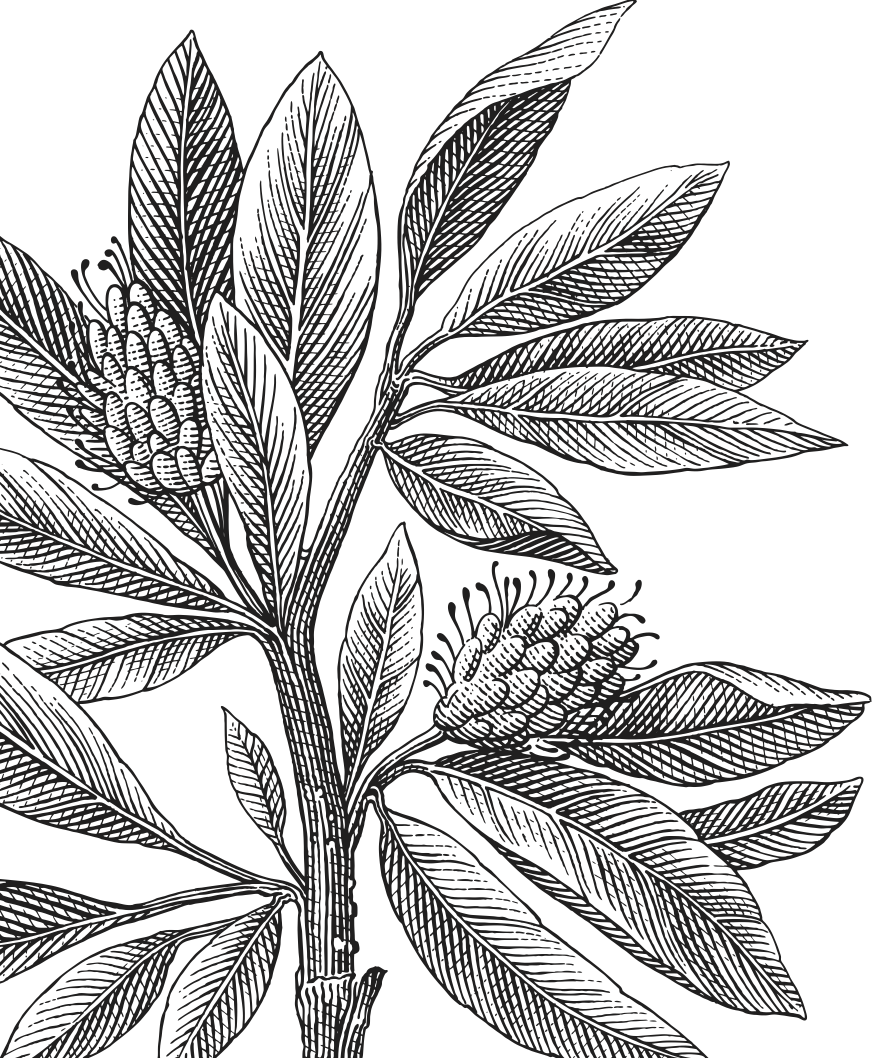
\includegraphics[keepaspectratio,scale=0.3]{img/lnu_etch.png} % Background picture
    }
}
\newcommand\BackgroundPicLogo{
    \put(30,740){
    
\includegraphics[keepaspectratio,scale=0.10]{img/logo.png} % Logo in upper left corner
    }
}

\title{	
\vspace{-8cm}
\begin{sidebar}
    \vspace{10cm}
    \normalfont \normalsize
    \Huge Report \\
    \vspace{-1.3cm}
\end{sidebar}
\vspace{3cm}
\begin{flushleft}
    \huge Project Course In Computer Science\\ 
    \it \LARGE - Team 3 first Seminar
\end{flushleft}
\null
\vfill
\begin{textblock}{6}(10,13)
\begin{flushright}
\begin{minipage}{\textwidth}
\begin{flushleft} \large
\emph{Author:} Quasim Aljubarah, Michael Johansson, Tadas Lisauskas, Zeyuan Li, Robin Reijo and Robin Stempa\\ % Author
\emph{Supervisor:} Ola Petersson\\ % Supervisor
%\emph{Examiner:} Dr.~Mark \textsc{Brown}\\ % Examiner (course manager)
\emph{Semester:} VT 2016\\ % 
\emph{Subject:} 1DV508\\ % Subject area
\end{flushleft}
\end{minipage}
\end{flushright}
\end{textblock}
}

\date{} 

\begin{document}
\pagenumbering{gobble}
\newgeometry{left=5cm}
\AddToShipoutPicture*{\BackgroundPic}
\AddToShipoutPicture*{\BackgroundPicLogo}
\maketitle
\restoregeometry
\clearpage

\selectlanguage{english}

\tableofcontents

\newpage
\pagenumbering{gobble}
\pagenumbering{arabic}

%----------------------------------------------------------------------------------------
%
%	Here follows the actual text contents of the report.
%
%----------------------------------------------------------------------------------------
\section{Introduction}
Second week's to-do list was to update the first weeks  website design and to update the document with functionality/analysis for the webshop. 

\section{Products And Categories}
We have to main category that is "Computers and misc" where we are going to sell some pre built computers and laptops, some monitors and also hardware/software so our categories on the page will be the following: 
\begin{itemize}
	\item{Monitors}
	\subitem{less than 24"}
	\subitem{24-27"}
	\subitem{larger than 27"}
	
	\item{Computers}
	\subitem{Asus}
	\subitem{MSI}
	\subitem{etc.}
	
	\item{Laptops}
	\subitem{Asus}
	\subitem{MSI}
	\subitem{etc.}
	
	\item{Computer Components}
	\subitem{Graphics cards}
		\subitem{Hard drives}
		\subsubitem{SSD}
		\subsubitem{Mechanical}
	\subitem{Processors}
	\subitem{etc.}
	
	\item{Software}
	\subitem{Windows}
	\subitem{Anti-virus}
	\subitem{Adobe}
	
	\item{Accessories}
	\subitem{Keyboards}
	\subitem{Mice}
	\subitem{Headphones}
	\subitem{etc.}
	
\end{itemize}

\section{Website Design Sketch}
The website will be similar to most of the web shops. Having a search bar, products/categories list, add to cart button, checking every product, adding to cart and administrator login button.

Administrator view will have extra buttons on all of the same pages and some of the bars changed to edit (instead of add to cart).

\subsection{Regular View}
\begin{figure}[htbp]
	\caption{Homepage}
	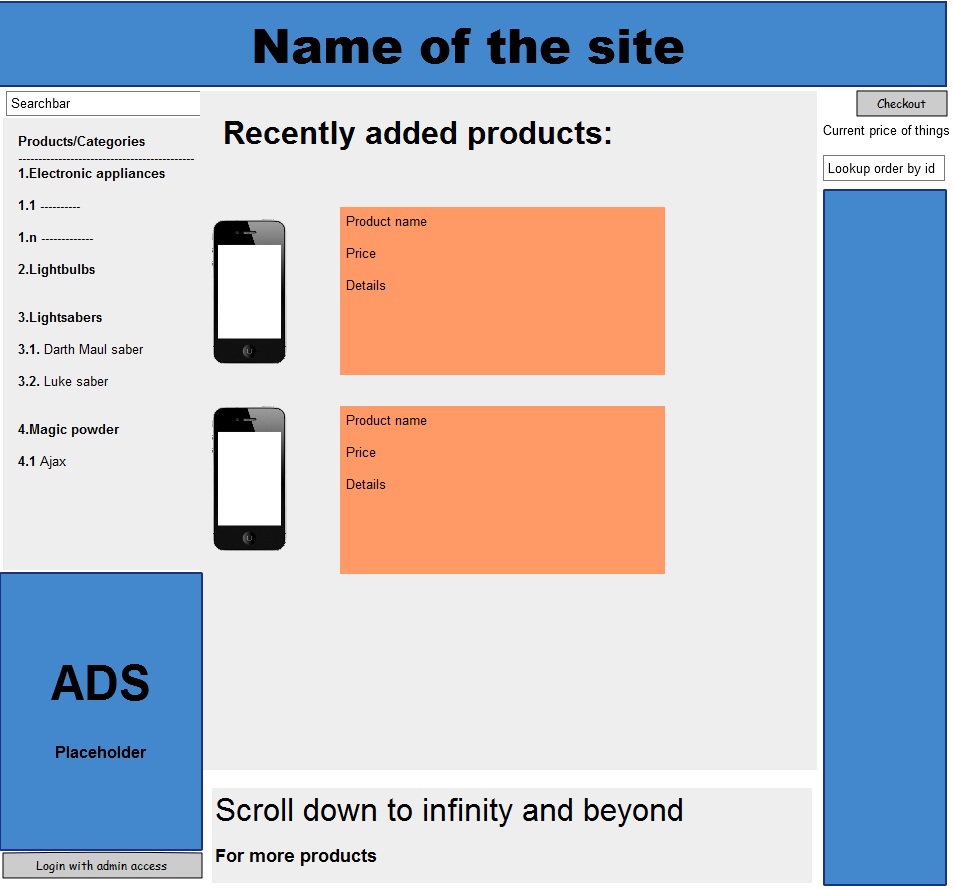
\includegraphics[width=\textwidth,height=\textheight,keepaspectratio]{img/Homepage.png}
\end{figure}

\begin{figure}[htbp]
	\caption{Product view}
	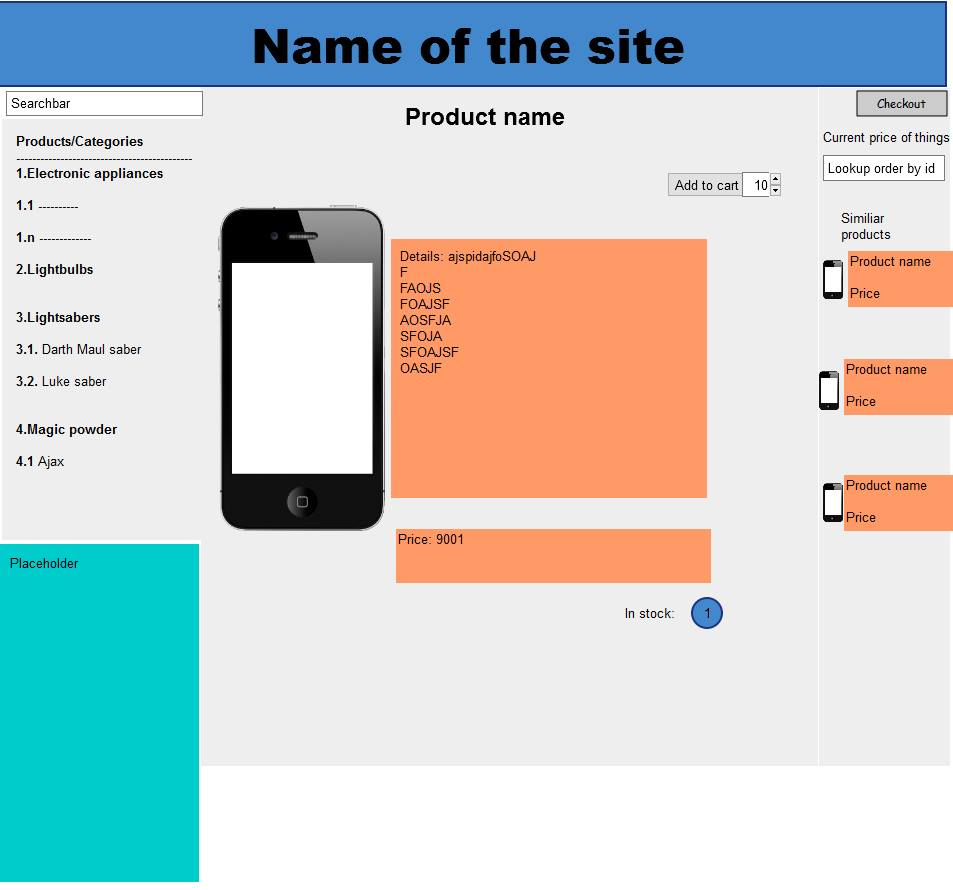
\includegraphics[width=\textwidth,height=\textheight,keepaspectratio]{img/Product_view.png}
\end{figure}

\begin{figure}[htbp]
	\caption{Checkout}
	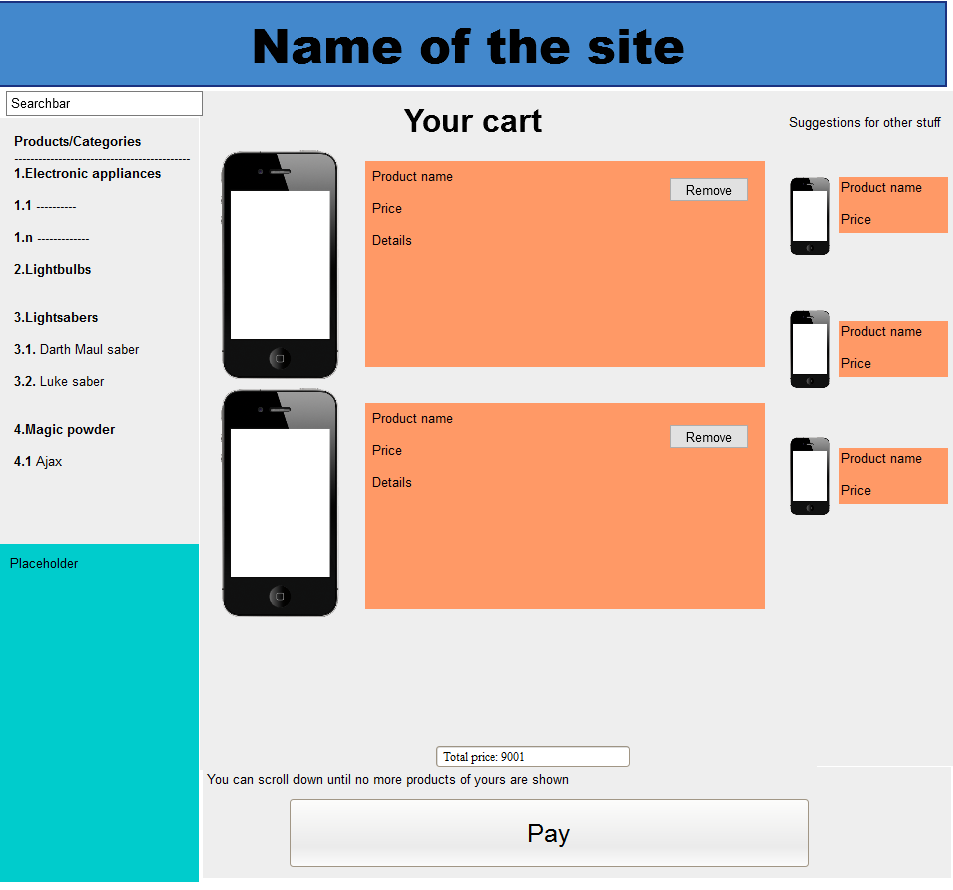
\includegraphics[width=\textwidth,height=\textheight,keepaspectratio]{img/Checkout.png}
\end{figure}

\begin{figure}[htbp]
	\caption{Search}
	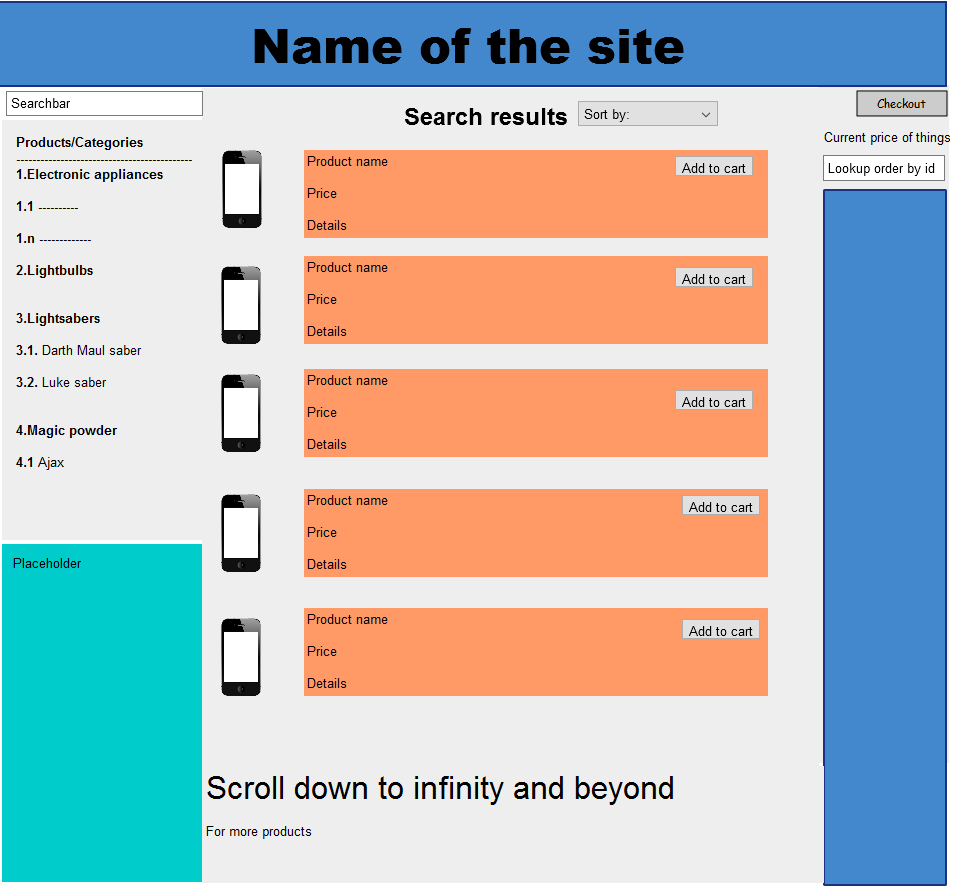
\includegraphics[width=\textwidth,height=\textheight,keepaspectratio]{img/Search.png}
\end{figure}

\newpage
\subsection{Administrator view}

\begin{figure}[htbp]
	\caption{Admin homepage}
	\includegraphics[width=\textwidth,height=\textheight,keepaspectratio]{img/Admin_Homepage.png}
\end{figure}

\begin{figure}[htbp]
	\caption{Admin product view}
	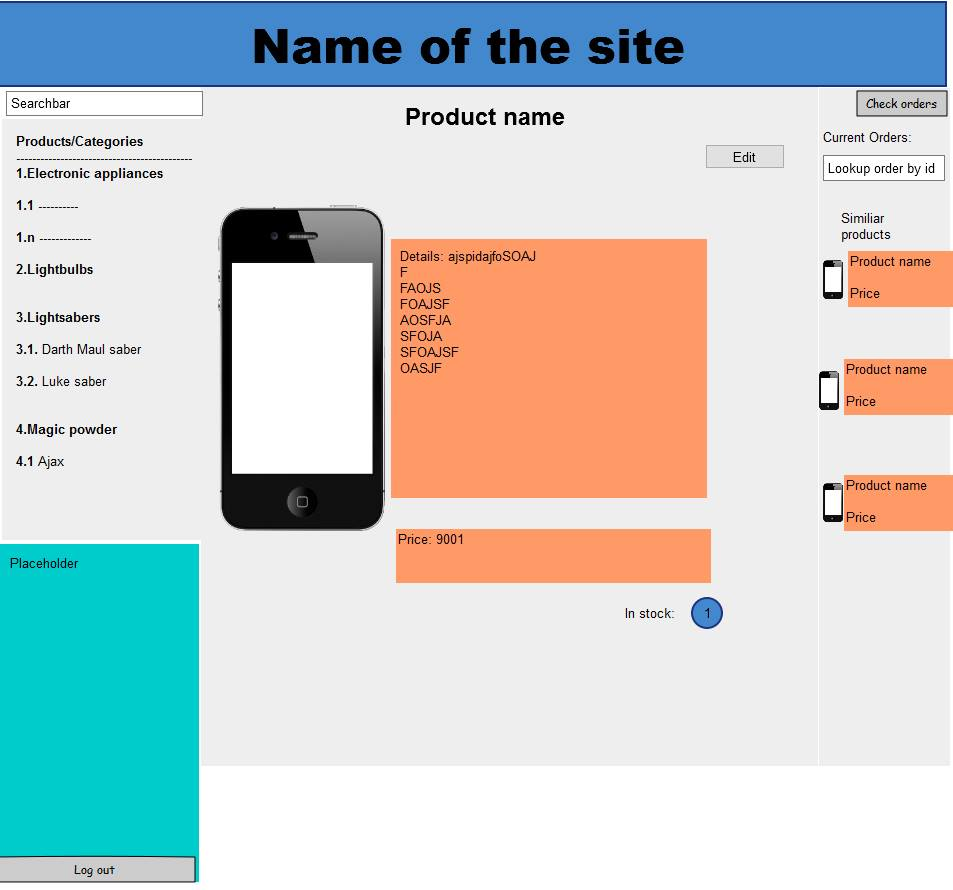
\includegraphics[width=\textwidth,height=\textheight,keepaspectratio]{img/Admin_product.png}
\end{figure}

\begin{figure}[htbp]
	\caption{Admin order management}
	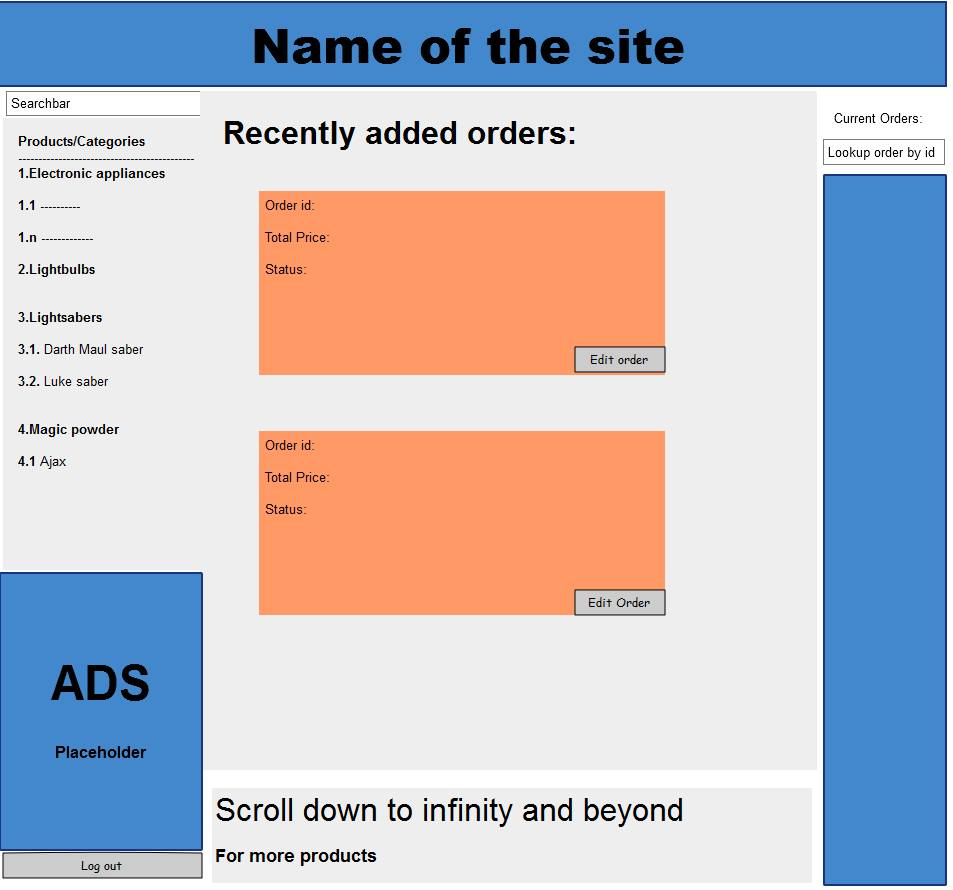
\includegraphics[width=\textwidth,height=\textheight,keepaspectratio]{img/Admin_order.png}
\end{figure}

\begin{figure}[htbp]
	\caption{Admin products view}
	\includegraphics[width=\textwidth,height=\textheight,keepaspectratio]{img/Products_admin.png}
\end{figure}
\newpage
\section{Analysis}
This section will cover all the requirements for the webshop and define them.
\subsection{General requirements }
This table analyses the general requirements for the webshop.
\newline

	\begin{tabular}{|l|l|}
		\hline
		ID  & Requirement                                                                                                                              \\ \hline
		1   & The webshop shall contain any number of products.                                                                                        \\ \hline
		1.1 & All information about the products shall be stored in the database.                                                                      \\ \hline
		1.2 & \begin{tabular}[c]{@{}l@{}}Each product will have:\\ -Product name\\ -Category\\ -Quantity\\ -Price\\ -Description\\ -Image\end{tabular} \\ \hline
		1.3 & All products will be pre-defined to categories (Monitors,Computers, Etc.                                                                 \\ \hline
	\end{tabular}
\subsection{Customer requirements}
This table will look into the customer requirements
\newline

	\begin{tabular}{|l|l|}
		\hline
		ID  & Requirement                                                                                                                                                                                      \\ \hline
		2   & \begin{tabular}[c]{@{}l@{}}The customer shall be able to browse the products in the\\ following ways:\\ -Browse all products\\ -Search for a product\\ -Show products in a category\end{tabular} \\ \hline
		2.1 & \begin{tabular}[c]{@{}l@{}}It shall be possible to click on a product to see more details\\ about it.\end{tabular}                                                                               \\ \hline
		2.2 & \begin{tabular}[c]{@{}l@{}}The customer shall be able to put a product in a Shopping\\ Basket.\end{tabular}                                                                                      \\ \hline
		2.3 & \begin{tabular}[c]{@{}l@{}}The customer shall be able to view the products in the\\ Shopping Basket.\end{tabular}                                                                                 \\ \hline
		2.4 & \begin{tabular}[c]{@{}l@{}}It shall be possible to change the quantity of a product in the\\ Shopping Basket, or remove a product.\end{tabular}                                                   \\ \hline
		2.5 & The customer shall be able to place an order   .                                                                                                                                                  \\ \hline
		2.6 & \begin{tabular}[c]{@{}l@{}}When placing an order, a form shall be shown where the\\ customer enters his/her contact details (email, address, phone\\ number). \end{tabular}                        \\ \hline
		2.7 & \begin{tabular}[c]{@{}l@{}}When an order is finalized the customer shall receive an auto-generated\\ order number. \end{tabular}                                                                    \\ \hline
		2.8 & \begin{tabular}[c]{@{}l@{}}The customer shall be able to check the status of his/her order\\ from the order number.\end{tabular}                                                                  \\ \hline
	\end{tabular}
\subsection{Administrator requirements}
Last section will look into the requirements for the administrator view mode and the functionalities it must have.
\newline

	\begin{tabular}{|l|l|}
		\hline
		3    & \begin{tabular}[c]{@{}l@{}}The webshop shall have an Admin system where an\\ administrator can log in.\end{tabular}                                                                          \\ \hline
		3.1  & User accounts and passwords shall be stored in the database.                                                                                                                                 \\ \hline
		3.2  & \begin{tabular}[c]{@{}l@{}}When a customer places an order, the order shall be added tothe database and the quantity of the ordered products shall be\\ updated in the webshop.\end{tabular} \\ \hline
		3.3  & It will be possible to add a new product.                                                                                                                                                    \\ \hline
		3.4  & It will be possible to remove a product.                                                                                                                                                     \\ \hline
		3.5  & It will be possible to change information about a product.                                                                                                                                   \\ \hline
		3.6  & It will be possible to manage deliveries (i.e. update the quantity of items).                                                                                                                \\ \hline
		3.7  & It will be possible to add a new administrator account.                                                                                                                                      \\ \hline
		3.8  & It will be possible to to remove an administrator account.                                                                                                                                   \\ \hline
		3.9  & It will be possible to add a new product category.                                                                                                                                           \\ \hline
		3.10 & It will be possible to view all orders.                                                                                                                                                      \\ \hline
		3.11 & It wil be possible to update an order.                                                                                                                                                       \\ \hline
		3.12 & Each order shall have a status: New, Delayed or Shipped                                                                                                                                      \\ \hline
		3.13 & An administrator will have to  update the order status manually.                                                                                                                             \\ \hline
	\end{tabular}

\subsection{UML Design}
The preliminary UML design is in the picture below.
\begin{figure}[htbp]
	\caption{UML Design}
	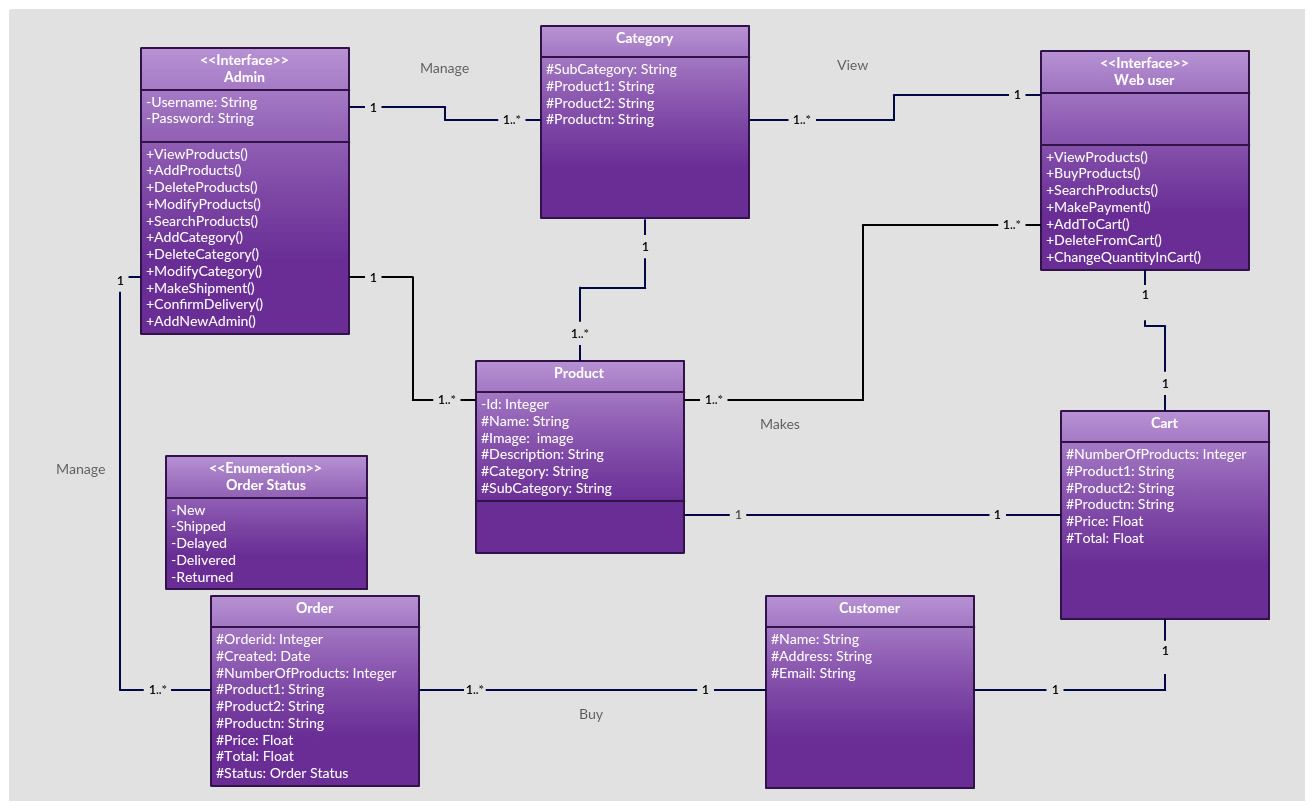
\includegraphics[width=\textwidth,height=\textheight,keepaspectratio]{img/UML.png}
\end{figure}
\end{document}
